\subsection{多候选精修：多结构候选与模拟筛选}
\subsubsection{从图结构形成不同粒度的划分}
单一粒度难以同时处理长链、宽层和大量独立分量。宽层中的细粒度 Task 可以分摊到多个核心，窄层或关键主链若切得过细，却会反复承担 DDR 中转与任务间隔。多候选精修因此构造一组有明确结构依据的划分，而不是只在结构感知搜索所得划分附近作扰动。所有划分仍覆盖每个非 COPY 算子且不重叠，并在加入每核序后检查扩展商图无环。

以原图拓扑层深 $d(v)$ 和层宽 $w_d$ 描述并行结构：
\begin{equation}\label{eq:q1-layer-depth}
d(v)=1+\max_{u\in\operatorname{pred}(v)}d(u),\qquad
w_d=|\{v:d(v)=d\}|,\qquad\max\varnothing=0.
\end{equation}
沿拓扑深度形成粗、细两档窗口；窄层主干采用较粗窗口，宽层及分支采用较细窗口。程序同时枚举若干层宽与深度阈值，保留完整弱连通分量、混合链、按张量字节划分和容量受控批次等候选。主导分量可被拆分，彼此独立的小分量则可按计算 Pipe 负载组合。窗口只是生成合法子图的候选规则，不能由层宽直接推导实际完成时间；被切断的张量还要按共同模型计入中转与等待。

为给任务放置提供较廉价的局部时间尺度，设子图 $r$ 各 Pipe 的估计工作量为 $W_{r,p}$，使用“最长 Pipe 加总工作量补偿”或经核内成本校准的代理：
\begin{equation}\label{eq:q1-allin-proxy}
\widehat\tau_r^{(a)}=\max_p W_{r,p}+0.08\sum_p W_{r,p},\qquad
\widehat\tau_r^{(b)}=\omega\max_p W_{r,p}+(1-\omega)\sum_p W_{r,p}.
\end{equation}
权重 $\omega$ 随候选设置变化，反映 Pipe 重叠程度的不同近似。该式是调度代理，既不宣称是总时长下界，也不以代理最优替代模拟最优。多候选精修保留这些不同代理，是为了在同一真实事件模型下检验它们提出的结构是否有效。

\subsubsection{预计完成时间与后继代价引导的放置}
对每个候选商图，从汇点反向计算任务的后续工作量，以关键任务优先的列表调度构造核心映射。基础放置采用 HEFT 型最早完成时间思想\cite{topcuoglu}：在满足数据释放和同核顺序的可插入位置中选择预计完成较早者。带前瞻的候选还计入后继任务的估计代价，以避免当前任务局部完成较早，却把后继链放到不利的核心。此处的前瞻表仅作排序，跨核释放仍遵循式\eqref{eq:q1-release}，共享 DDR 的最终争用由官方事件模拟计算。

与结构感知搜索的单个配置最多 $12$ 次完整评价不同，多候选精修先保留基础候选，再追加结构层候选，按划分、映射和顺序的规范指纹去重。其五核扩展包括额外层结构及局部搜索；这些设置不能直接当成一至四核均已验证的算法收益。设候选集合为 $\mathcal C_0$，模拟阶段求
\begin{equation}\label{eq:q1-allin-choice}
p_0=\arg\min_{p\in\mathcal C_0\cap\mathcal P_A(k)}
\operatorname{lex}\bigl(T_i^A(p),D_i(p)\bigr).
\end{equation}
由于 $\mathcal C_0$ 并不保证包含结构感知搜索的最终解，多候选精修不存在逐图必优保证；即使百图均值提高，仍需检查逐图退步。

\subsubsection{五核局部改进与算法步骤}
五核局部搜索以已评价最优方案为起点，保持子图划分，尝试核心迁移、交换和保持拓扑合法的核心顺序调整。若修改不满足覆盖或无环条件，直接拒绝；若官方模拟的字典序目标不改善，不替换当前最优。局部步数随图规模递减，超过 $9000$ 个计算操作时跳过该扩展，以限制大图代价。历史运行设置了局部阶段 $600$ 秒墙钟界限，并以已发生的构造评价成本决定是否进入局部搜索；这不是整个冷启动流程的 $600$ 秒保证。

算法的完整步骤如下。
\begin{enumerate}
\item 读取图及硬件配置，计算拓扑层、弱连通分量、主链、Pipe 工作量与共享张量关系。
\item 生成完整分量、粗细窗口、混合链和容量批次等划分，分别用基础及带前瞻的列表调度映射到核心。
\item 去除重复与非法候选，逐一调用官方内层排程与共享 DDR 事件模拟，按式\eqref{eq:q1-allin-choice}保存实测最优。
\item 五核配置在规模和时间条件允许时，对固定划分执行迁核、交换与顺序邻域搜索，更新实测最优。
\item 输出子图归属与每核顺序；独立恢复并回放保存的方案，核对周期和额外搬运，不把恢复历史方案的时间作为全新搜索时间。
\end{enumerate}
记结构候选数为 $M$，局部提案数为 $L$，一次构造、合法性检查和官方评价成本分别为 $C_g,C_v,C_e$，则总成本可写为
\begin{equation}\label{eq:q1-allin-complexity}
O\bigl(M(C_g+C_v+C_e)+L(C_v+C_e)\bigr).
\end{equation}
固定候选的商图无环检查为 $O(q+|E_\pi|)$；$C_e$ 还受核内准备、溢出和在途事件数量影响，不能笼统写成只依赖节点数的常数。因此多候选精修的主要代价来自更丰富的候选及相应模拟，并未消除大图评价瓶颈。

\subsection{两种方案的比较与适用范围}
\subsubsection{完整核数曲线}
多候选精修的一至四核补跑及独立复核已完成，现与五核已核实组合共同组成100图、1至5核的500组结果。图\ref{fig:q1-complete}将两方法按相同算例及固定单核分母对齐。多候选精修的五点平均加速比分别为1.000000、1.860204、2.604827、3.272613和4.026824；多核均值均高于结构感知搜索，但三核总周期为110359308，高于后者的109880862。说明逐图等权的平均收益不能替代整批图的周期比较。五核沿用已恢复核对的交付组合，低核采用本次补跑结果；本图不构成全部配置等预算重新搜索的实验。

\begin{figure}[!htbp]\centering
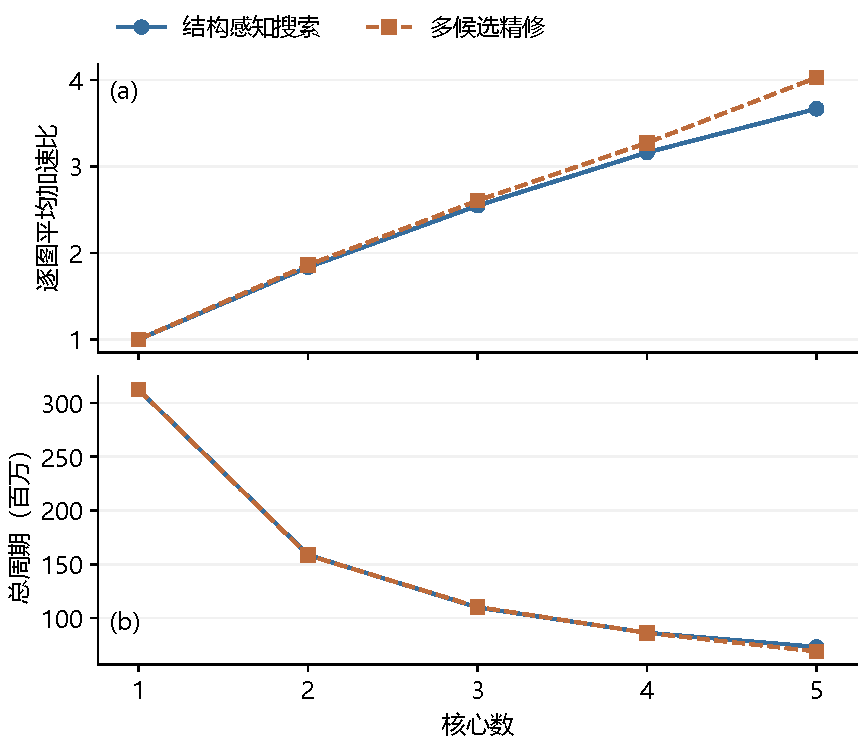
\includegraphics[width=0.92\linewidth,height=0.70\textheight,keepaspectratio]{../图表/runs/20260926-A-six-figures/fig_q1_complete_curves.pdf}
\caption{两种方法在100图、1至5核下的平均加速比与总周期}\label{fig:q1-complete}\label{fig:q1-speed}\label{fig:q1-total}
\end{figure}
\subsubsection{相同单核分母下的五核结果}
采用相同的 $100$ 张输入图及同一官方评价语义，将两种方案逐图配对。结构感知搜索取已交付的 r02 结果；多候选精修取 Allin2 最新交付组合，并恢复全部 $100$ 份五核方案作官方回放。两批逐图单核分母逐项一致，恢复结果的完成周期及额外搬运均与保存的交付摘要一致。该核对支持输出结果比较，不代表重新实施了等预算的算法实验。
\begin{table}[!htbp]\centering
\caption{问题一两种方案的百图五核配对比较}\label{tab:q1-two-methods}
\begin{tabular}{lrr}
\toprule
指标 & 结构感知搜索 & 多候选精修\\
\midrule
逐图平均加速比 & 3.665903 & 4.026824\\
总完成周期（cycles） & 73170501 & 68905422\\
总额外搬运（bytes） & 1767728284 & 1807542424\\
配对图数 & 100 & 100\\
\bottomrule
\end{tabular}
\end{table}
多候选精修相对结构感知搜索为 66 胜、21 平、13 负，胜负按完成周期判断。平均加速比相对提高 9.85\%，总完成周期下降 5.83\%。前一指标对每图等权，后一指标更受大图影响，二者不可互换；多候选精修的总额外搬运反而增加约 2.25\%，表明其周期收益并非来自总搬运量的整体减少，而与并行安排及关键等待有关。搬运作为次级指标单列，不替代完成周期。

图\ref{fig:q1-case-gains}按五核逐图周期改善率从小到大排列全部100个算例，改善率定义为“结构感知搜索周期减多候选精修周期”，再除以结构感知搜索周期。横轴是排序位置而非原始算例编号，负值完整保留。多数改善集中于一部分图，仍有13个退步例，故不能把平均改善解释为逐图支配。

\begin{figure}[!htbp]\centering
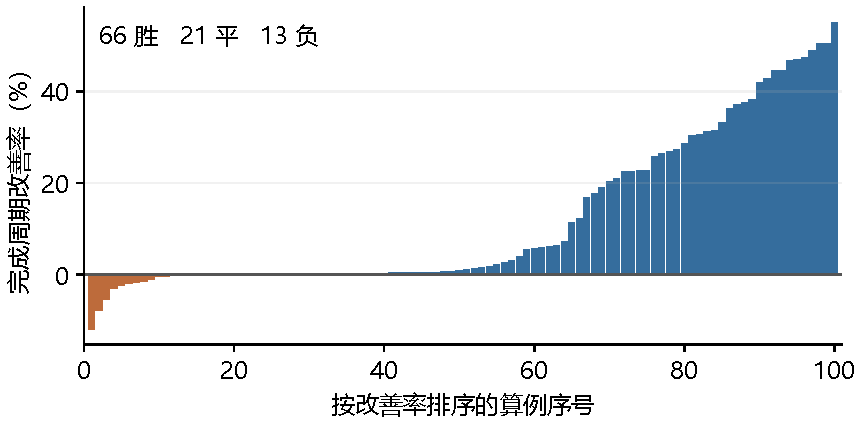
\includegraphics[width=0.92\linewidth,height=0.70\textheight,keepaspectratio]{../图表/runs/20260926-A-six-figures/fig_q1_case_gains.pdf}
\caption{五核逐图完成周期改善率分布}\label{fig:q1-case-gains}
\end{figure}
\subsubsection{性能收益与计算预算的边界}
结构感知搜索把评价机会限制为 $12$，适合昂贵模拟条件下的稳定基线。多候选精修覆盖更多层结构和映射候选，能改善整体五核结果，但历史全量搜索平均约 $708.98$ 秒、最长约 $3371.6$ 秒，$49$ 张图的搜索评价时间超过 $600$ 秒。这些历史统计来自全量搜索记录，并非本次恢复过程或最新交付组合的端到端计时；交付摘要还组合了不同阶段的已得方案。因此，当前对照能说明最终交付质量差异，不能单独归因于变宽划分、前瞻放置或局部搜索中的某一项。

若硬性限制在线求解资源，宜先采用结构感知搜索作为可复核基线，再在统一评价次数与统一墙钟预算下比较多候选精修。若允许离线充分搜索，可采用多候选精修已核实的五核组合。一至四核结果现已独立复核并纳入完整核数曲线，但仍需等预算消融和端到端计时，才能判断不同机制的独立收益。两种方案均为有限候选启发式，未证明全局最优。

